%!TEX root = ../dokumentation.tex

\chapter{Durchführung  der Probandenversuche} 
Im folgenden Kapitel werden die geplanten Probandenversuche und deren Durchführung genauer erklärt. Während der Bearbeitung der Arbeit hat sich die grundlegende Situation jedoch so sehr geändert, dass eine Durchführung, wie geplant, nicht stattfinden konnte. Mehr hierzu in \autoref{section:corona}.

\section{Probleme der Probandenversuche}
\label{section:corona}
Die Durchführung dieser Arbeit war für den Zeitraum November 2019 bis Juni 2020 vorgesehen. Die Durchführung der Probandenversuche war in der ursprünglichen Planung für April 2020 angesetzt. Allerdings wurden durch die Corona-Pandemie \cite{rki.2020} Kontaktbeschränkungen beschlossen, die eine Durchführung in geplanter Größenordnung erschweren. Ursprünglich wurde mit einer Teilnehmerzahl von runde 20 Probanden geplant. Leider war es nicht möglich den Versuch in dieser Größenordnung durchzuführen. Alle Daten, die erhoben wurden, sind von zwei Probanden und den Autoren selbst erstellt. Dies beeinflusst die Messergebnisse enorm, sodass keine klaren Rückschlüsse und somit keine eindeutige Antwort auf die Forschungsfrage gegeben werden kann. Die beiden folgenden Kapitel werden unter Berücksichtigung dieser Einschränkung die vorhandenen Daten auswerten und anhand derer probieren, erste Aussagen über die Eignung von Eye-Tracking zur Steuerung in VR zu treffen.

\section{Versuchsaufbau} 
In \autoref{section:versuchsumgebung} wird der Aufbau der unterschiedlichen Level bereits erklärt. Es ergeben sich folgende Kombinationsmöglichkeiten für einen Versuchsaufbau:
\begin{itemize}
	\item 4 verschiedene Umgebungen
	\item 2 unterschiedliche Formen des Anvisierens (Laserpointer/Controller und Eye-Tracking)
	\item 2 unterschiedliche Formen des Auswählens (Triggerbetätigung und Blinzeln)
	\item 3 unterschiedliche Größen für die Knöpfe
\end{itemize}
Daraus lässt sich berechnen wie viele verschiedene Aufbauten A es insgesamt gibt:
\begin{align}
	A=4*2*2*3=48
\end{align}
Um erste Indizien geben zu können, sollen für jeden möglichen Versuchsaufbau fünf Messungen zur Verfügung stehen. Das bedeutet, dass insgesamt mindestens 240 Messungen durchgeführt werden sollten. Dabei soll jeder Proband alle Steuermöglichkeiten gleich oft testen. Das bedeutet, dass bei 20 Probanden jeder Proband zwölf Messungen durchführt. Jeweils drei sind eine Steuermöglichkeits-Kombination. Diese drei Versuche werden nach folgendem Muster entworfen:
\begin{enumerate}
	\item Das erste Level ist eine der vier Steuermöglichkeiten mit einer zugeteilten Distanz und einer zugeteilten Knopfgröße.
	\item Das zweite Level verändert die Distanz zu den Objekten, behält aber die Knopfgröße und die Steuerart bei.
	\item Das dritte Level verändert die Größe des Knopfes, behält aber Steuerart und Distanz vom ersten Level bei.
	\item Dieses Muster wiederholt sich vier mal - für jede Steuerart ein mal.
\end{enumerate}
Mit dieser Methode ist es möglich, alle unterschiedlichen Parameter möglichst gleichmäßig zu testen. Da jeder Proband einen unterschiedlichen Ablauf hat, werden Lerneffekte und andere unerwünschte Nebeneffekte neutralisiert. Mit einem Plan, wie in \autoref{table:probanden} beschrieben, würde jeder Testaufbau mit fünf Versuchen getestet werden. Durch die Veränderung eines einzelnen Parameters zwischen jedem Versuch lässt sich der Einfluss jedes Parameters in mehreren Testaufbauten messen. Im \autoref{table:probanden} ist die verwendete Testreihe gezeigt. Jede Zeile beschreibt einen Probanden. Die Anordnung der Tabelle ist zufällig generiert und hilft so mögliche Lerneffekte oder Ähnliches zu verhindern. Die Daten in der Tabelle geben für jeden der 20 Probanden zwölf Versuche an. Ein Versuch ist als Tupel von zwei Zahlen angegeben. Es werden immer drei Versuche pro Proband gemacht. Ein Tupel (x, y) beschreibt als x die Größe der Knöpfe und als y das gewählte Level. Der Parameter x hat drei Stufen, eins bis drei, wobei eins der größten Größe entspricht und drei der kleinsten. Bei y beschreiben die Werte eins bis drei die unterschiedliche Distanz zu den Objekten, bzw. das dementsprechende Level. Bei y=1 sind die Knöpfe sehr nah, bei y=3 sind sie weit weg. Bei y=4 wird das 3D-Level genutzt. Hier variiert die Distanz der Knöpfe je nach Knopf. 

\subsection{Ablauf eines Probandenversuchs}
Der Probandenversuch findet in Gruppenterminen statt. Dabei werden nach und nach Probanden benötigt. Da wegen Hardwareeinschränkungen nicht zeitgleich getestet werden kann, wird ein Zeitplan entworfen. Jeder Proband kommt einzeln in den Testraum. Hier werden zunächst allgemeine Informationen gesammelt. Dazu gehören Alter, Erfahrung mit VR und ob der Proband eine Sehhilfe nutzt. Daraufhin wird dem Nutzer die VR-Brille aufgesetzt und die grundsätzlichen Einstellungen (zum Beispiel das Anpassen der Bänder am Kopf) werden vorgenommen. In einer Beispielumgebung wird dem Proband das Prinzip des Versuchs erklärt. Die Augen werden für das Eye-Tracking kalibriert. Wenn der Proband sich bereit für den Versuch fühlt, werden nach und nach die entsprechenden Level geladen und bewältigt. Die Messdaten werden automatisch erfasst und zur Auswertung gespeichert. Die Daten und Auswertung sind in den \autoref{section:results} und \autoref{section:discussion} zu sehen. Sobald der Proband die für ihn bestimmten zwölf Versuche durchgeführt hat, füllt er einen Fragebogen (siehe \autoref{section:fragebogen}) aus. Die Ergebnisse und Auswertung dieser werden in den Abschnitten \autoref{section:resultquestions} und \autoref{section:discussionquestions} erläutert.

Aufgrund der \ac{COVID-19}-Pandemie wurden die Probandenversuche jedoch angepasst. Anstatt 20 Probanden wurde die Zahl auf vier reduziert. Zwei dieser Probanden waren die Autoren der Arbeit selbst. Außerdem wurden die Versuchsanzahl deutlcih reduziert und die Variation unter den Versuchen auf wesentliche Aspekte beschränkt. Jede Steuermethode wurde mit einer festen Distanz mit jeweils großen und kleinen Knöpfen von jedem Proband untersucht. Dadurch ergeben sich acht unterschiedliche Versuchsaufbauten, die jeder Proband einmal durchläuft. Die Reihenfolge der Versuche war bei jedem Proband gleich. 

\subsection{Teilnehmer der Studie}
Die Teilnehmer der Studie waren zwei Probanden und die beiden Autoren der Arbeit.
\begin{itemize}
	\item Proband 1: männlich, 20 Jahre, keine Sehhilfe, regelmäßiger VR-Nutzer, kein vorheriger Kontakt mit der Arbeit, studiert Mechatronik
	\item Proband 2: männlich, 21 Jahre, Kontaktlinsen, regelmäßiger VR-Nutzer, Autor der Arbeit, studiert Informatik/IT-Automotive
	\item Proband 3: männlich, 24 Jahre, Brille (während der Versuche ohne Sehhilfe), mehrere Erfahrungen mit VR, Autor der Arbeit, studiert Informatik/IT-Automotive
	\item Proband 4: männlich, 21 Jahre, keine Sehhilfe, sehr wenig Erfahrung mit VR, kein vorheriger Kontakt mit der Arbeit, studiert Medizintechnik
\end{itemize}

\section{Fragebogen} 
\label{section:fragebogen}
Der Fragebogen stellt einen wichtigen Teil in der Beantwortung der Forschungsfrage dar. Das Ziel dieser Arbeit ist es, herauszufinden, ob sich Eye-Tracking für die Steuerung in VR eignet. Dafür ist das subjektive Empfinden der Nutzer enorm wichtig. Mit den Messwerten aus den Versuchen lassen sich zwar Parameter wie Schnelligkeit vergleichen, allerdings ist die subjektive Empfindung bei Eingabegeräten immer ein wichtiger Faktor. Deshalb soll der Fragebogen die Frage beantworten, welche Steuermöglichkeit von den Probanden bevorzugt wird und warum die Steuermöglichkeit bevorzugt wird.
\subsection{Fragen}
Der Fragebogen besteht aus zwei Teilen: Einerseits werden Fragen zu jeder Steuermöglichkeit separat gefragt, andererseits werden Fragen zum allgemeinen Empfinden und den Steuermöglichkeiten im Vergleich gefragt.
Zu jeder Steuermöglichkeit wird gefragt, :
\begin{itemize}
	\item wie leicht die Fixierung und das Auswählen des richtigen Knopfes gefallen ist.
	\item wie gut wie gut der Proband sich eine Steuerung mit dieser Konfiguration vorstellen kann.
	\item wie stark eine Veränderung der Distanz und der Größe der Knöpfe einen Einfluss auf die Steuerung hat.
\end{itemize}
Am Ende der Befragung wird der Proband gebeten, ein begründetes Ranking der Steuermöglichkeiten abzugeben. Hier können auch offene Punkte angemerkt werden, die nicht im restlichen Teil des Fragebogens abgefragt werden.


\section{Ergebnisse der Versuche}
\label{section:results}
Im Folgenden werden die gemessenen Ergebnisse der Probandenversuche dargestellt. 
\subsection{Vergleich der Steuermöglichkeiten}
\label{section:comparison}
Zuerst werden die Gesamtzeiten und die Fehlerquote der Steuermethoden miteinander verglichen. Anschließend wird überprüft, welche Auswirkung eine Verkleinerung der Knöpfe auf diese beiden Werte hat. Anschließend wird der Einfluss des Abstandes zwischen den Knöpfen betrachtet und abschließend werden die Blickdaten der Probanden betrachtet.
\subsubsection{Gesamtdauer}
In \autoref{fig:totalTimesBig} ist die Dauer eines Versuches von jedem Probanden und die durchschnittliche Dauer pro Steuermöglichkeit zu sehen. Hier lässt sich erkennen, dass mit der Kombination Laserpointer/Trigger die Versuche am schnellsten abgeschlossen wurden. Diese haben im Durchschnitt 7,724 Sekunden in Anspruch genommen. Der schnellste Versuch hat 6,432 Sekunden gedauert und der langsamste Versuch hat 10,954 Sekunden benötigt.

\begin{figure}[!htbp]
	\centering
	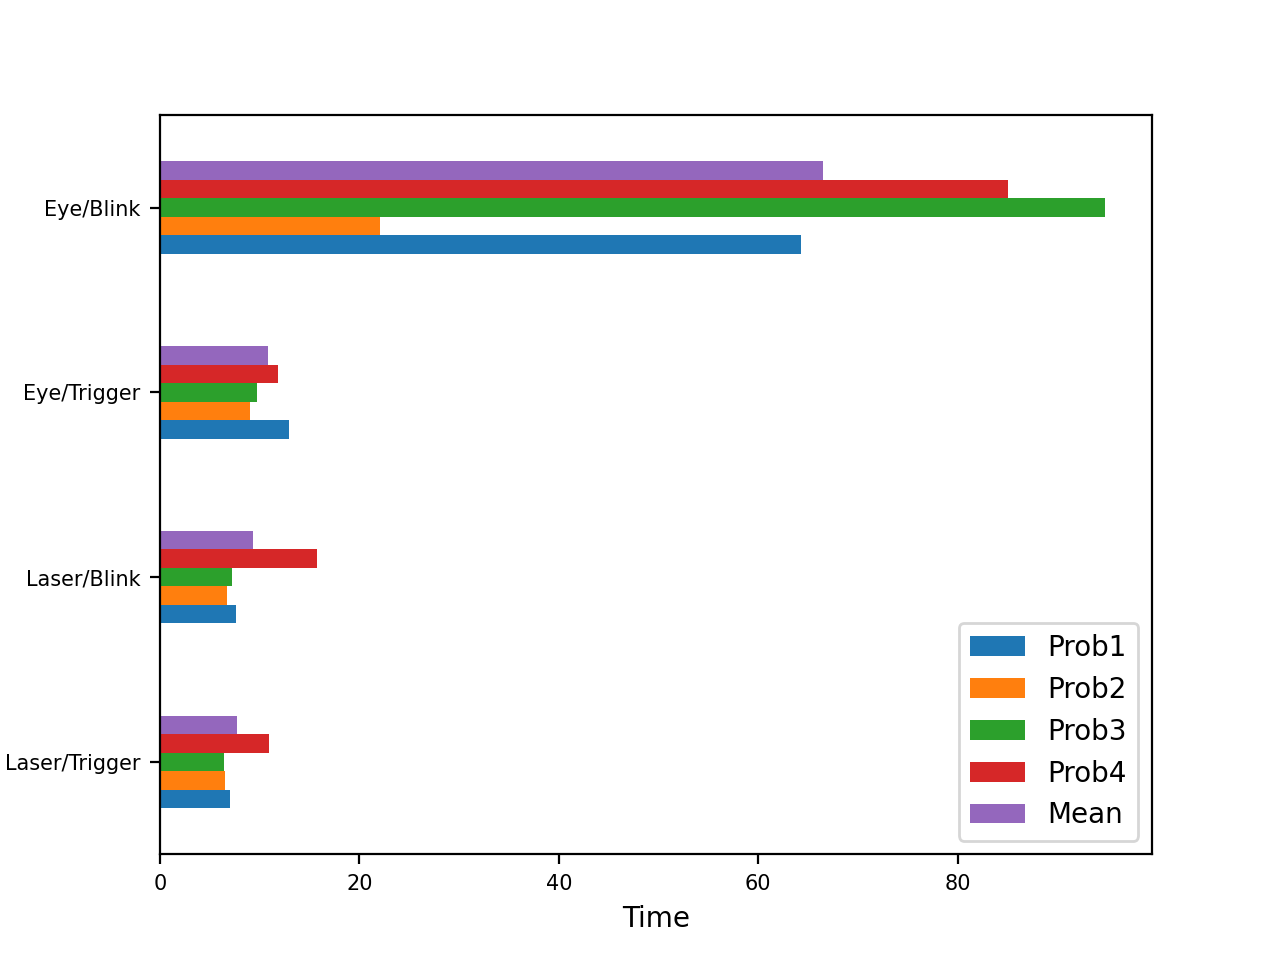
\includegraphics[width=0.8\linewidth]{plot_big}
	\caption[Gesamtdauer eines Versuchdurchlaufs pro Steuerart pro Proband und im Durchschnitt]{Gesamtdauer eines Versuchdurchlaufs pro Steuerart pro Proband und im Durchschnitt}
	\label{fig:totalTimesBig}
\end{figure}

Die Kombination Laserpointer/Blinzeln hat die zweitschnellsten Ergebnisse geliefert. Hier haben die Probanden im Durchschnitt 9,305 Sekunden benötigt. Der schnellste Versuch lag bei 6,674 Sekunden und der langsamste bei 15,748 Sekunden. 

Beim Einsatz der Steuermethode Eye-Tracking/Trigger lag die durchschnittliche Zeit, bis ein Versuch beendet wurde, bei 10,877 Sekunden. Hier hat der schnellste Versuch 9,026 Sekunden benötigt, der langsamste Versuch lag bei 12,924 Sekunden.

Bei der Kombination von Eye-Tracking/Blinzeln haben Versuche deutlich länger gedauert. Im Schnitt lagen die Probanden hier bei 66,549 Sekunden um die fünf richtigen Knöpfe auszuwählen. Ein Proband schaffte es deutlich schneller mit 22,116 Sekunden, zwei Probanden haben deutlich länger gebraucht, mit Zeiten von 85,063 und 94,761 Sekunden

\subsubsection{Genauigkeit}

\begin{figure}[!htbp]
	\centering
	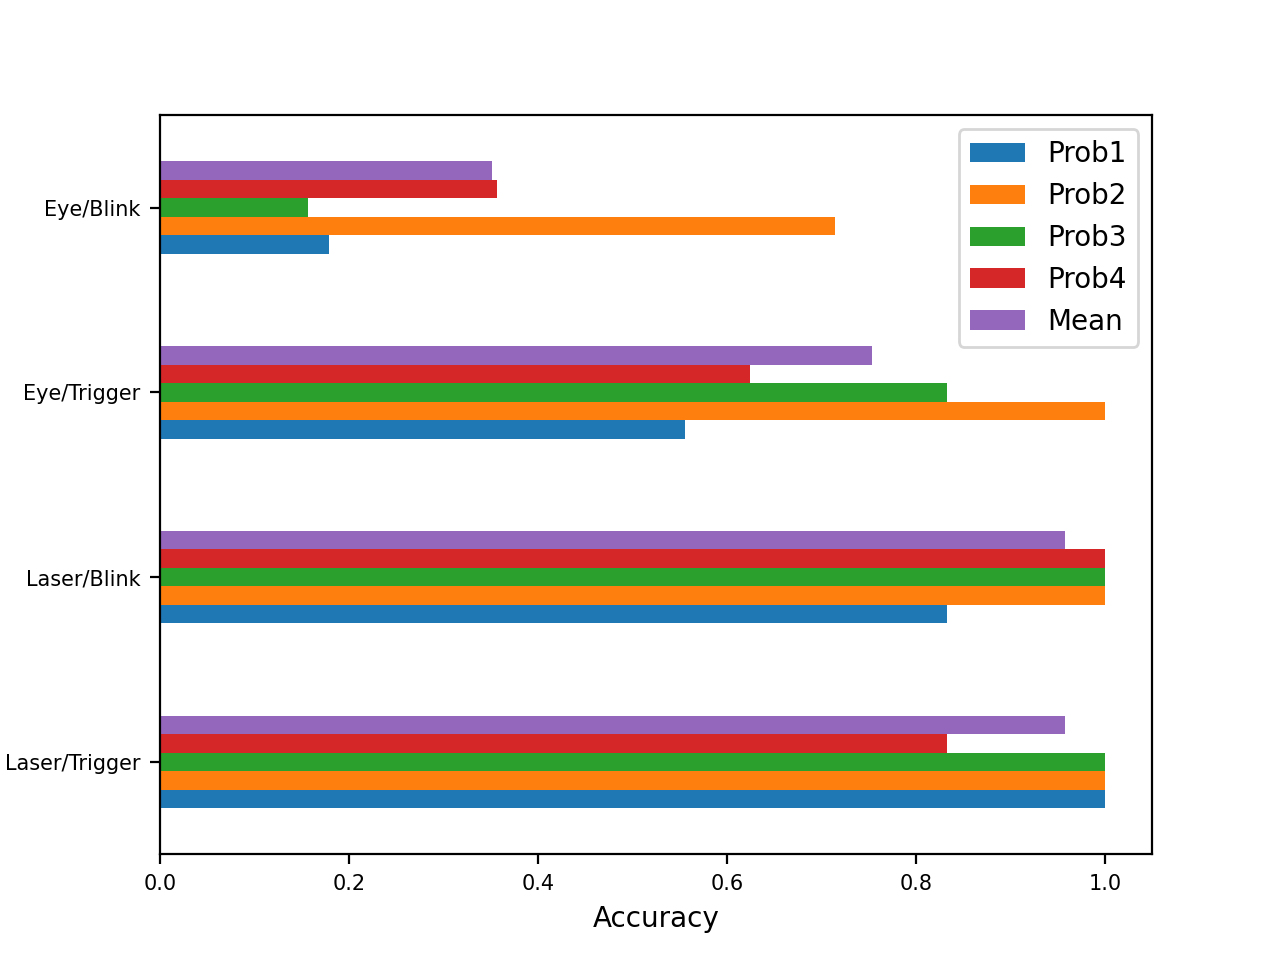
\includegraphics[width=0.8\linewidth]{plot_acc_big}
	\caption[Anteil der richtigen Angaben pro Steuerart pro Proband und im Durchschnitt]{Anteil der richtigen Angaben pro Steuerart pro Proband und im Durchschnitt}
	\label{fig:totalACCBig}
\end{figure}
In \autoref{fig:totalACCBig} ist die Genauigkeit der Eingaben der Probanden zu sehen. Die Werte stellen den Anteil der Eingaben dar, bei denen der richtige Knopf getroffen wurde. Hier ist zu erkennen, dass  für den Laserpointer sowohl beim Blinzeln zum Bestätigen, als auch beim Trigger eine sehr hohe Genauigkeit vorliegt. Im Durchschnitt haben die Probanden eine Genauigkeit von 95,83\% erreicht, wobei bei beiden Steuermethoden die schlechteste Genauigkeit 83,3\% beträgt. Das entspricht einer falschen Eingabe auf fünf richtige Eingaben.

Bei der Steuermethode Eye-Trackin/Trigger ist die durchschnittliche Genauigkeit nur noch 75,35\%. Hier hat Proband 2 als einziger noch 100\% Genauigkeit bewerkstelligen können, Proband 1 ist mit einer Genauigkeit von 55,55\% am ungenausten. 

Beim Einsatz von Eye-Tracking/Blinzeln zum Bestätigen betrug die durchschnittliche Genauigkeit nur noch 35,15\%. Proband 2 hat auch hier wieder die höchste Genauigkeit mit 71,42\%. Bei den anderen Probanden ist die Genauigkeit auf bis zu 15,63\% gefallen. 



\subsection{Einfluss der Veränderung der Knopfgröße}
\label{section:influencebuttonsize}
In diesem Abschnitt wird zuerst auf die Veränderung der Gesamtzeit mit einer Verkleinerung der Knöpfe auf 50\% der ursprünglichen Breite und danach die Auswirkung auf die Genauigkeit betrachtet. 
\subsubsection{Gesamtdauer}
In \autoref{fig:timesIncrease} sind die Veränderungen der Gesamtzeiten der Versuche pro Steuermethode und pro Proband und dem Mittelwert bei einer Verkleinerung der Breite des Knopfes um 50\% als Faktor dargestellt. Ein Faktor größer eins bedeutet folglich eine längere Dauer, ein Faktor unter eins bedeutet eine kürzere Dauer. Im Durchschnitt ist bei jeder Steuermethode ein Faktor größer eins, also eine erhöhte Dauer pro Versuch, zu sehen. Bei der Steuermethode Laserpointer/Trigger kam es zu einem Anstieg von 22\%. Proband 2 war hier als einziger schneller (um 5\%), als in dem selben Versuch mit größeren Knöpfen. Er hat im Versuch mit kleinen Knöpfen nur 6,714 Sekunden benötigt. Proband 4 hat mit einem Anstieg von 92,7\% fast doppelt so lange gebraucht, wie im selben Versuch mit großen Knöpfen. Bei Proband 1 ist ein Anstieg von 35\% zu einer Gesamtzeit von 9.494 Sekunden aufgetreten.

\begin{figure}[!htbp]
	\centering
	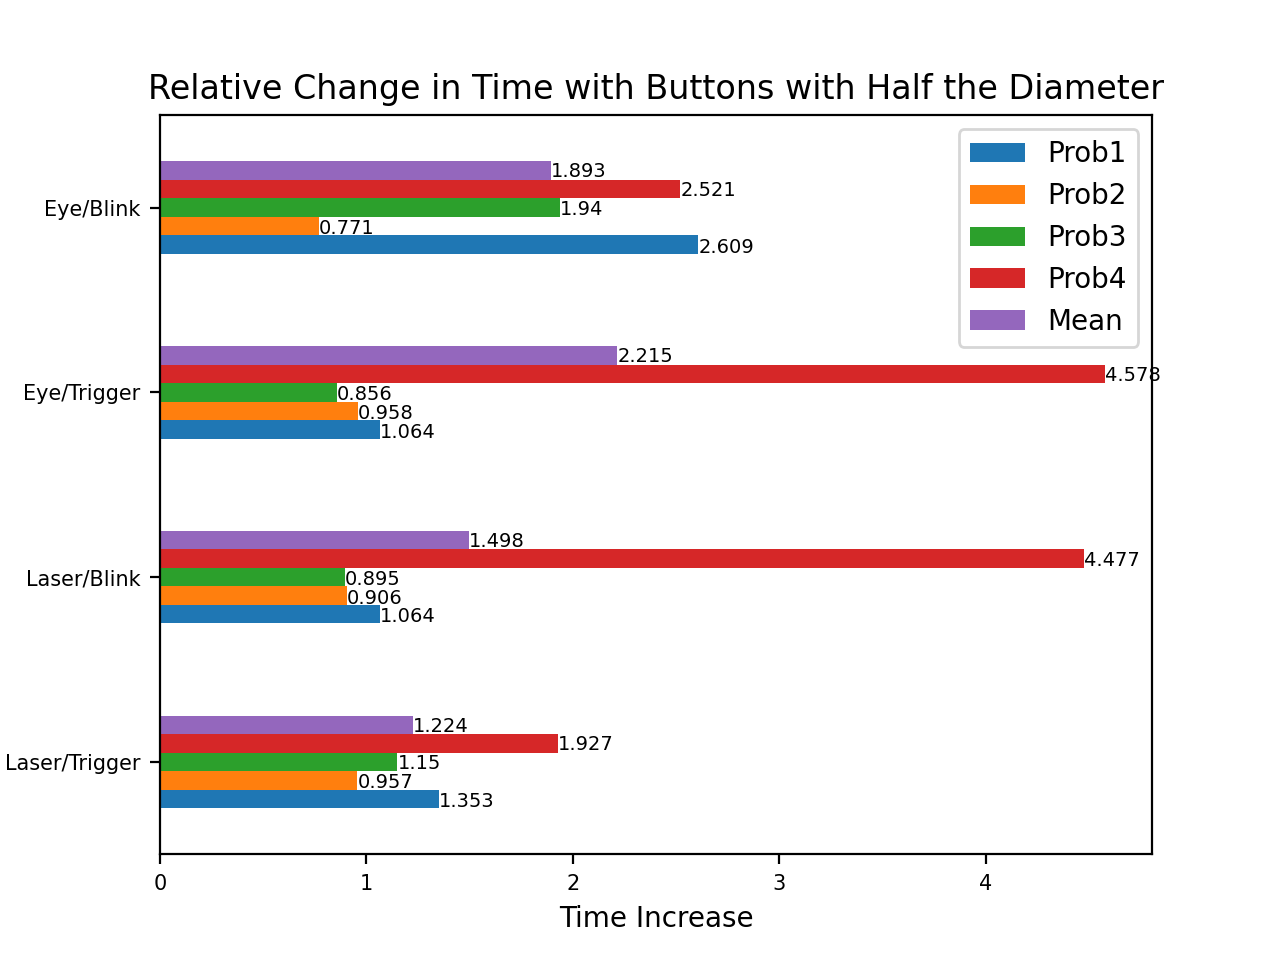
\includegraphics[width=0.8\linewidth]{plot_time_increase}
	\caption[Anteil der richtigen Angaben pro Steuerart pro Proband und im Durchschnitt bei kleineren Knöpfen]{Anteil der richtigen Angaben pro Steuerart pro Proband und im Durchschnitt bei kleineren Knöpfen}
	\label{fig:timesIncrease}
\end{figure}

In den Hybrid-Steuermethoden (Laserpointer/Blinzeln und Eye-Tracking/Trigger) ist die durchschnittliche Dauer um 49,76\%, bzw 121,4\% angestiegen. Im Durchschnitt lag die Zeit für die beiden Steuermethoden somit bei 13,936  und 24,091 Sekunden. Probanden 2 und 3 haben hier jeweils einen Wert besser als 1,0 erzielt, waren also schneller als mit großen Knöpfen. Proband 3 war im Versuch Laserpointer/Blinzeln 11\% (Gesamtzeit 6,794 Sekunden) schneller und im Versuch Eye-Tracker/Trigger 15\% (Gesamtzeit 11,069 Sekunden) schneller als im selben Versuch mit größeren Knöpfen. Proband 4 hat auch in diesen beiden Steuermethoden einen starken Anstieg der Gesamtzeit im Vergleich zum selben Versuch mit größeren Knöpfen. Hier lagen die Werte bei 447\% und 457\%, was in Gesamtzeiten von 33,996 und 59,160 Sekunden resultierte. Die Gesamtdauer ist damit auch deutlich über den anderen Probanden, die hier im Durchschnitt nur 7,249 und 12,401 Sekunden benötigt haben. Proband 1 hat in beiden Steuermethoden rund 6,3\% länger gebraucht, als im selben Versuch mit größeren Knöpfen. Dies resultierte in den Zeiten 8,077 Sekunden für Laserpointer Blinzeln und 13,75 Sekunden für Eye-Tracking/Trigger.


Bei der Steuermethode Eye-Tracking/Blinzeln kam es im Durchschnitt zu einem Anstieg der Gesamtdauer von 89\%. Die Gesamtdauer für diese Steuermethode stieg somit auf 125.952 Sekunden. Der einzige Proband, der eine Verbesserung im Vergleich zu großen Knöpfen erreicht hat, war Proband 2. Dieser hat das Level 23\% schneller erledigt, als mit großen Knöpfen. Das entspricht einer Zeit von 49.559 Sekunden. Proband 1 hat eine Änderung von 160\% auf 167.622 Sekunden verzeichnet. Bei Proband 3 stieg die Zeit um 93,97\% auf 124.641 Sekunden und bei Proband 4 betrug der Anstieg 152\% auf 161.987 Sekunden. 

\subsubsection{Genauigkeit}
In \autoref{fig:totalACCsmall} ist die Genauigkeit der Steuermethoden pro Proband und im Durchschnitt bei einer Verkleinerung der Knöpfe zu sehen. Für die Steuermethode Laserpointer/Trigger ist die durchschnittliche Genauigkeit von rund 96\% bei den großen Knöpfen auf nur noch 74\% abgesunken. Proband 2 hat als einziges eine Genauigkeit von 100\%, bei allen anderen Probanden sind Fehler aufgetreten. Proband 1 ist von 100\% Genauigkeit im Versuch mit großen Knöpfen auf nur noch 62,5\% abgerutscht. Die schlechteste Genauigkeit hatte Proband 4 mit 50\%. Dieser hatte zuvor noch eine Genauigkeit von 83,33\%. Die durchschnittliche Genauigkeit ist bei der nächsten Steuermethode wieder gestiegen und hat hier den Wert 84,7\% erreicht. Bei großen Knöpfen wurde im Schnitt eine Genauigkeit von knapp 96\% erreicht. Proband 2 und 3 konnten, wie schon im Versuch mit den großen Knöpfen, 100\% Genauigkeit erreichen. Die schlechteste Präzision hatte Proband 1 mit 55,5\%, zuvor hatte er 83,3\%. Beim Einsatz von Eye-Tracking/Trigger zum Bestätigen wurde bei den kleinen Knöpfen eine durchschnittliche Trefferquote von 60,3\% erreicht. Zuvor lag dieser Wert bei 75,34\%. Die höchste Genauigkeit hatte in diesem Versuchsaufbau Proband 3, der seine Quote von 83,3\% von den großen Knöpfen halten konnte. Bei allen anderen Probanden ist die Genauigkeit gesunken. Proband 1 ist von 55\% auf 45\% abgerutscht, Proband 2 sogar von 100\% auf 62,5\%. Proband 4 ist von 62,5\% auf 50\% gesunken.

\begin{figure}[!htbp]
	\centering
	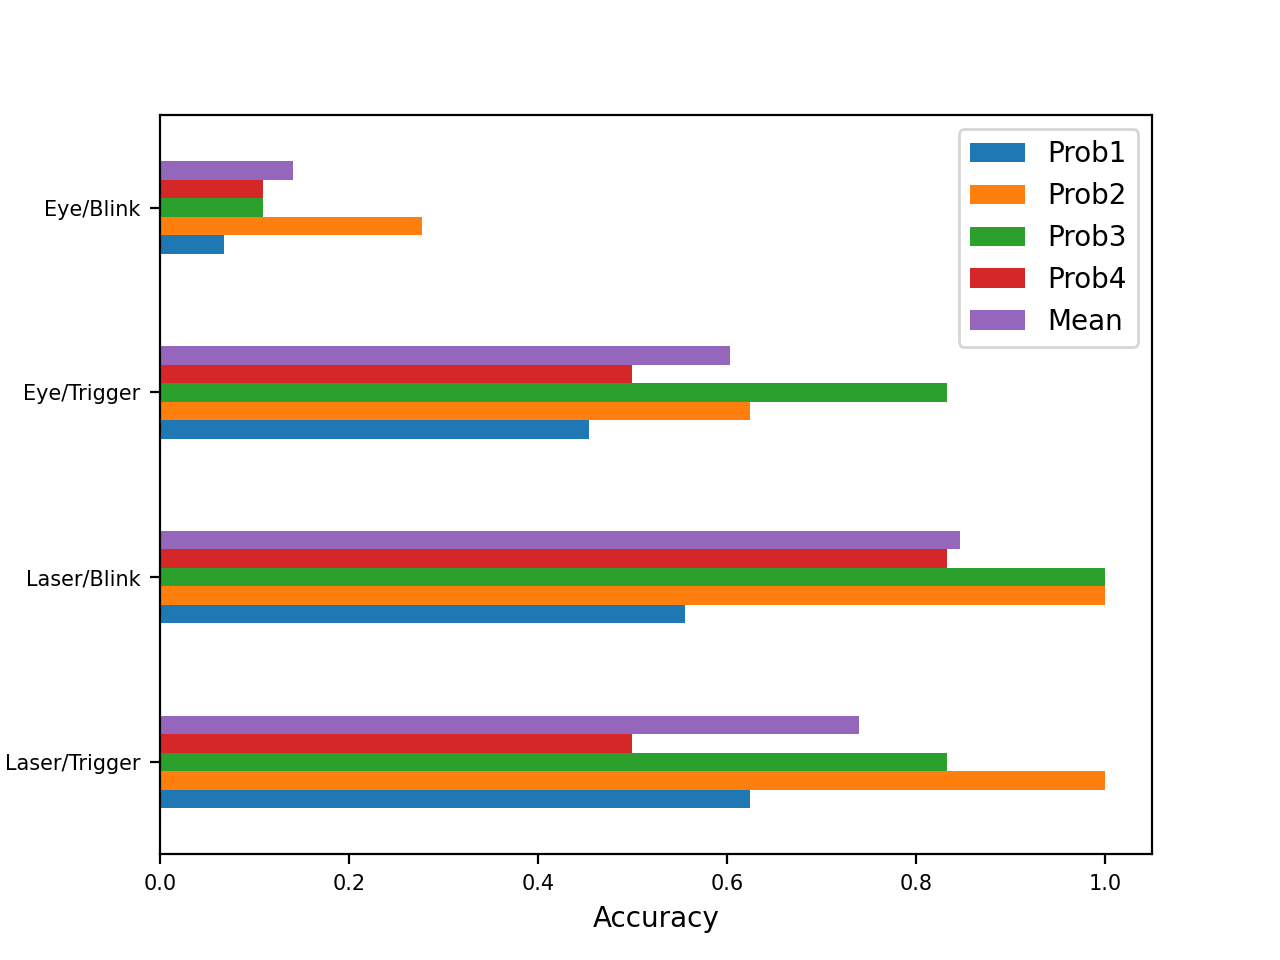
\includegraphics[width=0.8\linewidth]{plot_acc_small}
	\caption[Gesamtdauer eines Versuchdurchlaufs pro Steuerart pro Proband und im Durchschnitt mit kleinen Knöpfen]{Gesamtdauer eines Versuchdurchlaufs pro Steuerart pro Proband und im Durchschnitt mit kleinen Knöpfen}
	\label{fig:totalACCsmall}
\end{figure}

Bei der Steuermethode Eye-Tracking/Blinzeln sind die eh schon niedrigeren Werte der großen Knöpfe (35,15\% im Durchschnitt) noch weiter gesunken. Hier wurde im Durchschnitt nur noch bei 14\% der Eingaben der gewünschte Knopf getroffen. Besonders hervorstechend ist hier der Wert von Proband 1. Dieser hatte nur noch eine Trefferquote von 6,75\%, zuvor waren es noch 17,86\%. Proband 2 konnte mit 27,78\% die höchste Trefferquote aufweisen, zuvor hatte er jedoch noch eine Trefferquote von 71,42\%. Proband 3 und 4 konnten exakt die gleiche Genauigkeit von 10,86\% erreichen. Zuvor hatte Proband 3 15,625\% und Proband 4 35,71\% erreicht. 

\subsection{Einfluss der Veränderung der Distanz aller Knöpfe}
Der Einfluss einer Veränderung kann aufgrund des eingeschränkten Versuchsaufbaus nicht untersucht werden. In diesem Abschnitt würde ein Vergleich in den Zeiten und der Genauigkeit stattfinden.

\subsection{Einfluss der unterschiedlichen Distanzen zwischen den Knöpfen}
Die beiden variablen Parameter in Fitts' Gesetz sind die Distanz D und die Breite W (vgl. \autoref{section:FittsLaw}). Die Veränderung der Breite W wird in den Versuchen mit der Veränderung der Knopfgröße erreicht, die Distanz D wird über verschiedene Muster variiert (vgl. \autoref{section:game} \todo{JH: Stehen lassen bis Kapitel 4 fertig!!!!!!!!!!!!!!!!!!! haben wir sowas schon irgendwo? JH: Bis jetzt noch nicht wird aber denk in Game erklärt}). In \autoref{fig:plotbuttons} ist der Einfluss der unterschiedlichen Distanzen zwischen zwei Knöpfen auf die Zeit zwischen der Aktivierung zweier Knöpfe dargestellt. Die durchgezogenen Linien zeigen die tatsächlichen Werte, die gestrichelten Linien zeigen den Trend der Werte an. Damit wird überprüft, ob eine unterschiedliche Distanz zwischen Knöpfen auch zu einer unterschiedlichen Aktivierungszeit führt. Für die Daten wurden alle erfolgreichen Eingaben der Nutzer mit der Zeit und dem entsprechenden Knopf aufgezeichnet und analysiert. Daraus lässt sich die Distanz zwischen den Knöpfen und die benötigte Zeit berechnen. Da jeder Nutzer jeden Versuchsaufbau ein mal durchläuft, gibt es zu jeder Distanz mehrere Zeitwerte. Aus diesen Werten wird der Durchschnitt in \autoref{fig:plotbuttons} pro Versuchsaufbau dargestellt. Durch die geringe Probandenzahlen sind die Zahlen nur bedingt aussagekräftig, da die Distanz nur einer der Faktoren ist, die die \ac{MT} (vgl. \autoref{section:FittsLaw}) beeinflusst. Andere Faktoren, wie die Größe der Knöpfe oder die Erfahrung des Probanden mit Eye-Tracking und VR kann diese Werte deutlich stärker beeinflussen, als die Distanz alleine. Bei einer großen Zahl Probanden ist es wahrscheinlicher, dass sich diese Störfaktoren gegenseitig aufheben und so ein besserer Zusammenhang zwischen Distanz und Zeit erkennbar wird. 
\begin{figure}[!htbp]
	\centering
	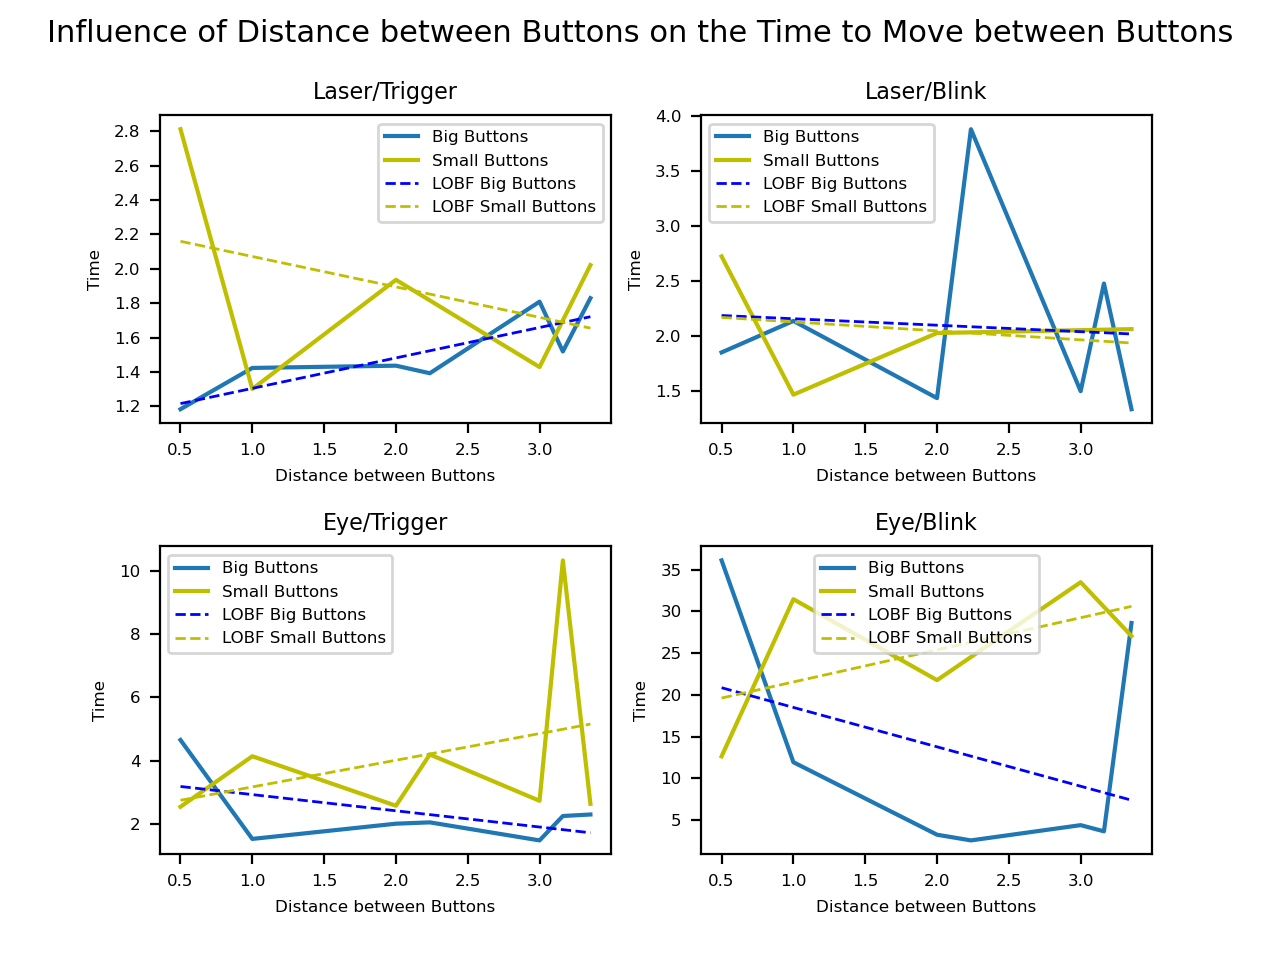
\includegraphics[width=0.8\linewidth]{plot_buttons}
	\caption[Einfluss der unterschiedlichen Distanzen zwischen zwei zu aktivierenden Knöpfen auf die Zeit, um beide Knöpfe zu aktivieren]{Einfluss der unterschiedlichen Distanzen zwischen zwei zu aktivierenden Knöpfen auf die Zeit, um beide Knöpfe zu aktivieren}
	\label{fig:plotbuttons}
\end{figure}
In jedem der vier Teilbilder ist eine Steuermethode dargestellt. Pro Steuermethode sind zwei Linien eingezeichnet, jeweils eine für große und eine für kleine Knöpfe. Bei der Steuermethode Laserpointer/Trigger mit großen Knöpfen ist eine Korrelation zwischen Distanz und Zeit zu erkennen. Hier steigt bei den großen Knöpfen die Zeit mit der Distanz zwischen den Knöpfen. So ist bei einer Distanz von 0,5\ac{u} die Zeit zwischen dem Aktivieren der beiden Knöpfe bei 1,184 Sekunden. Die Zeit steigt mit der Erhöhung der Distanz ebenso weiter an, wie an der Trendlinie zu erkennen ist. Bei den kleinen Knöpfen deutet die Trendlinie auf eine Abnahme der Zeit mit zunehmender Distanz hin. Allerdings ist hier der Wert für die kleinste Distanz (0,5\ac{u}) mit 2,812 Sekunden extrem hoch. Ohne diesen Wert ist auch hier ein Anstieg der Zeit mit einem Anstieg der Distanz zu erkennen. 

Bei der Steuermethode Laserpointer/Blinzeln sind die beiden Trendlinien fast identisch. Beide verlaufen mit einer minimal negativen Steigung. Hier hat eine Erhöhung der Distanz fast keinen Einfluss auf die Zeit zwischen dem Betätigen.

Bei der Steuermethode Eye-Tracking/Trigger sind die Trendlinien wieder stärker ausgeprägt. Allerdings würden beide Linien, sobald man den Wert mit der größten Abweichung von den anderen Werten nicht betrachtet, wieder so gut wie waagerecht verlaufen. Auch hier hat die Distanz fast keinen Einfluss auf die Zeit zwischen dem Betätigen. 

Die Trendlinien zur Steuermethode Eye-Tracking/Blinzeln weichen sehr stark voneinander ab. Bei großen Knöpfen schwanken die Zeiten zwischen dem Aktivieren zweier Knöpfe zwischen 2,588 Sekunden und 36,101 Sekunden.  Bei den kleinen Knöpfen schwanken die Werte zwischen 12,648 und 33,49 Sekunden und sind im Durchschnitt deutlich höher als die Werte für die großen Knöpfe. Wie schon bei den anderen beiden Versuchsaufbauten, scheint die Distanz hier nicht der ausschlaggebende Faktor zu sein.

\subsection{Auswertung der Blickdaten}
Zur Auswertung der Blickdaten werden die, wie in \autoref{section:measurement} beschrieben, aufgezeichneten Daten analysiert, um eine grafische Darstellung zu ermöglichen. In \autoref{fig:plotheatmapprob2} sind die Blickdaten von Proband 2 aus den Versuchen mit den Steuermethoden Eye-Tracking/Trigger und Eye-Tracking/Blinzeln mit jeweils großen und kleinen Knöpfen dargestellt. Im \autoref{appendix:heatmaps} sind die Heatmaps aller Probanden zu sehen. In diesem Abschnitt werden die Blickdaten anhand von Proband 2 näher betrachtet. 

\begin{figure}[!htbp]
	\centering
	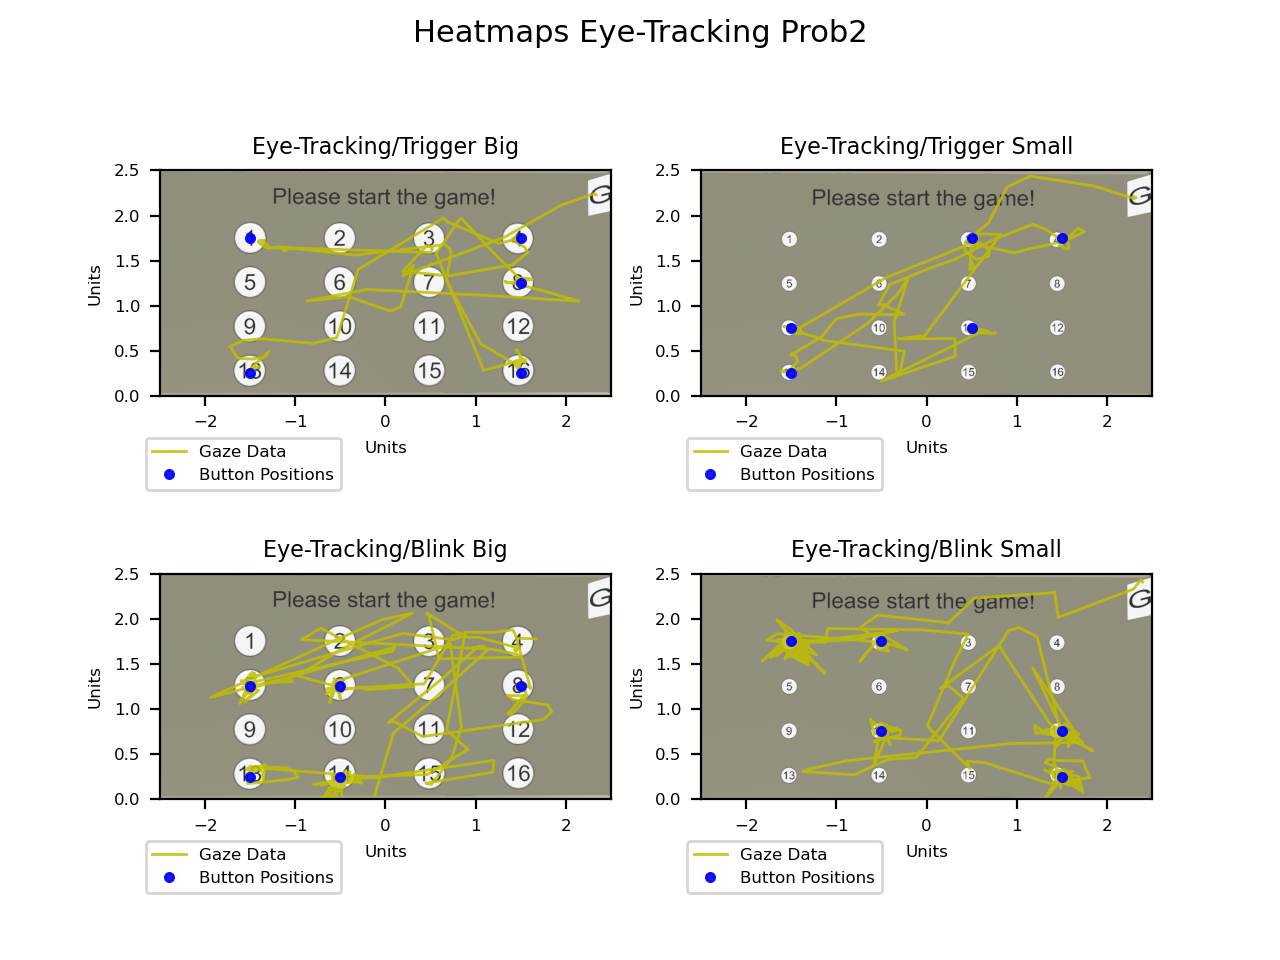
\includegraphics[width=0.8\linewidth]{plot_heatmap_prob2}
	\caption[Visualisierung der Blickdaten und der auszuwählenden Knöpfe] {Visualisierung der Blickdaten und der auszuwählenden Knöpfe}
	\label{fig:plotheatmapprob2}
\end{figure}

Die Blickdaten starten meist oben rechts, da sich an dieser Stelle der Go Button befindet. Beim Versuch Eye-Tracking/Blinzeln hat der Eye-Tracker keine Daten auf dem Go-Button aufgezeichnet, was darauf hindeutet, dass entweder in diesem Moment keine Daten gespeichert wurden, oder dass der Nutzer den Knopf gedrückt hat, ohne ihn direkt anzusehen. Der Blick des Probanden springt zwischen den Knöpfen stets nach oben zur Anzeige, um zu sehen, welcher Knopf als nächstes ausgewählt werden muss. Deshalb sind oft große Sprünge von einem Knopf in Richtung des Wortes \glqq game\grqq{} zu sehen. Je höher die Dichte der Striche um einen Knopf ist, desto länger hat der Proband seinen Blick auf diesen Knopf gerichtet, da mehr Daten des Eye-Trackers in diesem Gebiet aufgezeichnet wurden. Dies ist vor allem bei der Steuermethode Eye-Tracking/Blinzeln mit kleinen Knöpfen bei dem Knopf 1 zu sehen. Hier hat der Nutzer sehr lange seinen Blick auf diesen Knopf gerichtet. Das liegt daran, dass beim Blinzeln die Daten des Eye-Trackers kurzzeitig verfälscht werden und somit nicht mehr über dem Knopf liegen. Dadurch kommt es zu einer fehlerhaften Eingabe und der Nutzer muss erneut probieren, den Knopf zu treffen. Proband 2 war bei diesem Versuchsaufbau am schnellsten, weshalb hier im Vergleich zu den anderen Probanden (\autoref{appendix:heatmaps}) deutlich weniger Striche zu sehen sind. Bei den Blickdaten ist sehr gut die Ungenauigkeit, die durch vermehrtes Blinzeln auftritt, zu erkennen.

\section{Ergebnisse des Fragebogens}
\label{section:resultquestions}
Im Folgenden werden die Ergebnisse des Fragebogens dargestellt. Da jedoch eine Veränderung der Distanz aufgrund der \ac{COVID-19}-Pandemie nicht untersucht wurde, wurde diese Frage im Fragebogen nicht berücksichtigt. 

Im gesamten Ranking der Steuermöglichkeiten waren sich die Probanden grundsätzlich einig. Alle vier Probanden haben die Steuermethode Laserpointer/Trigger als die beste und Eye-Tracking/Blinzeln als die schlechteste Steuermethode angegeben. Bei drei der vier Probanden hat die Steuermethode Laserpointer/Blinzeln den zweiten und Eye-Tracking/Trigger den dritten Platz belegt. Bei einem Probanden waren diese beiden Steuermethoden vertauscht. In den folgenden Unterabschnitten werden die Ergebnisse zu den einzelnen Steuermöglichkeiten dargestellt und die Kommentare der Probanden aufgenommen. Die genauen Angaben der Probanden sind im \autoref{appendix:tables} zu finden.
\subsection{Laserpointer/Trigger}
Alle vier Probanden konnten den Sätzen \glqq Es fiel mir leicht, die richtigen Blöcke zu fixieren/auszuwählen\grqq{} und \glqq Ich kann mir eine Menüsteuerung mit dieser Methode vorstellen\grqq{} komplett zustimmen. Eine Veränderung der Knopfgröße hatte für alle vier Probanden \glqq ein wenig\grqq{} Einfluss auf die Fähigkeit, Knöpfe anzuvisieren und auszuwählen. Als Begründung für die erste Position im Ranking wurden vor allem Intuitivität und die einfache Gewöhnung an diese Steuermethode genannt. Den Nutzern ist sowohl das Anvisieren, als auch das Auswählen leicht gefallen. 
\subsection{Laserpointer/Blinzeln}
Diese Methode hat im Ranking bei drei von vier Probanden den zweiten Platz belegt. Dem Satz \glqq Es fiel mir leicht, die richtigen Blöcke zu fixieren\grqq{} konnten alle vier Probanden komplett zustimmen. Bei der Auswahl der Blöcke sind die Antworten sehr unterschiedlich ausgefallen. Der Proband, der diese Methode auf Rang 3 platziert hat, konnte der Aussage \glqq Es fiel mir leicht, die richtigen Blöcke zu auszuwählen\grqq{} nicht zustimmen. Die anderen Probanden konnten der Aussage größtenteils (2x) oder komplett (1x) zustimmen. Der Aussage \glqq Ich kann mir eine Menüsteuerung mit dieser Methode vorstellen\grqq{} konnte ein Proband komplett zustimmen, zwei Probanden konnten größtenteils zustimmen und der Proband, der Probleme mit dem Blinzeln zum Auswählen hatte konnte dieser Aussage gar nicht zustimmen. Eine Veränderung der Knopfgröße hatte für drei der vier Probanden einen geringen Einfluss, ein Proband stufte den Einfluss als normal ein. Die Begründung der drei Probanden, die diese Methode auf den zweiten Rang gesetzt hatten, nannten vor allem die gute Genauigkeit des Laserpointers als Grund für die hohe Platzierung. Das Blinzeln wurde zwar meist als gute Bestätigungsmethode genannt, einem Proband fiel es aber schwer, nicht aus Versehen an der falschen Stelle zu blinzeln. 
\subsection{Eye-Tracking/Trigger}
Beim Einsatz von Eye-Tracking in Verbindung mit dem Trigger des Vive Controllers konnte keiner der Probanden dem Satz \grqq Es fiel mir leicht, die richtigen Blöcke zu fixieren\grqq{} komplett zustimmen. Zwei der Probanden gaben an, der Aussage größtenteils zustimmen zu können, einer konnte teils zustimmen, einer nur ein wenig. Der Aussage \grqq Es fiel mir leicht, die richtigen Blöcke auszuwählen\grqq{} konnten alle Probanden größtenteils zustimmen. Zwei der Probanden konnten der Aussage \grqq Ich kann mir eine Menüsteuerung mit dieser Methode vorstellen\grqq{} komplett zustimmen, einer konnte größtenteils und einer teils zustimmen. Den Einfluss durch eine Veränderung der Knopfgröße beschreiben den Probanden als normal (1x) bis stark (3x). Ein Proband hat diese Methode als zweitbeste bewertet.
\subsection{Eye-Tracking/Blinzeln}
Diese Methode hat im Vergleich zu den anderen Methoden mit Abstand am schlechtesten abgeschnitten. Keinem der Probanden fiel es leicht die Blöcke anzuvisieren oder auszuwählen. Keiner der Probanden kann sich diese Steuermethode als Menüsteuerung vorstellen. Eine Veränderung der Knopfgröße hatte bei allen Probanden einen sehr starken Einfluss. Alle Probanden hatten das Problem, dass beim Blinzeln zum Bestätigen eines Knopfes der Eye-Tracker wieder verrutscht ist und somit keine genaue Steuerung möglich war.
